\chapter{抗逆向分析的PE文件保护技术}
\label{cha:sensorsys}

\section{PE文件格式}
\label{cha2:sec:PEfile}

本课题的任务内容是对PE文件进行修改并保护\cite{2017Compiler},然后使之可以正常运行,所以对于PE文件结构的内容不容忽视,由于PE文件的修改都是基本本章节内容,所以后文将会对本节内容进行多次引用,本章将会对本课题涉及到的关于PE文件结构进行详细的研究,并分析出PE文件可以经本课题使用的空间。
\subsection{PE文件总体结构}
本课题的目的是保护Windows的可执行程序,通过改变可执行文件的数据结构,防止被破解者分析篡改,所以一定要对Windows下的可执行程序有详细的了解,本节内容将会对PE文件进行详细分析,明确每个数据结构的作用,同时对有价值的信息进行保护\cite{2017A}。

PE(Portable Executable)是一种32位和64位Windodws下的可执行文件,包括后缀名为DLL和EXE等的可执行文件。PE格式是一种数据结构,其中封装了Windows OS加载程序管理包装的可执行代码所需的信息。这包括用于链接的动态库引用\cite{2018c},API导出和导入表,资源管理数据和线程本地存储TLS数据。在NT操作系统上,PE格式用于EXE,DLL,SYS设备驱动程序和其他文件类型。所述可扩展固件接口EFI规范规定PE是在EFI环境标准的可执行格式\cite{2018VMGuards}。与PE类似的格式是ELF,它在Linux和大多数其他版本的Unix中使用。
	
PE文件的一个非常方便的方面是磁盘上的数据结构与内存中使用的数据结构相同。可以通过调用LoadLibrary函数将可执行文件加载到内存中,遇到的问题主要如何将PE文件的某些范围数据映射到内存地址空间中。因此,像IMAGE\textunderscore NT\textunderscore HEADERS结构体这样的数据结构在磁盘和内存中是相同的。透彻了解PE文件结构中的内容,可以全面认识PE文件在执行时在内存中的布局\cite{2016Design}。
重要的是要注意,PE文件不只是作为单个内存映射文件映射到内存中。取而代之的是,Windows加载程序查看PE文件并决定要映射到文件的哪些部分。这种映射是一致的,因为当映射到内存时,文件中的较高偏移量对应于较高的内存地址。磁盘文件中项目的偏移量可能与加载到内存后的偏移量有所不同。但是,PE文件中的信息都会在系统内存中出现\cite{李路鹿2020代码混淆技术研究综述},以使您能够从磁盘偏移量转换为内存偏移量,如图\ref{sec2:subsec3:pememory}所示。

\begin{figure}[htbp]
	\centering
	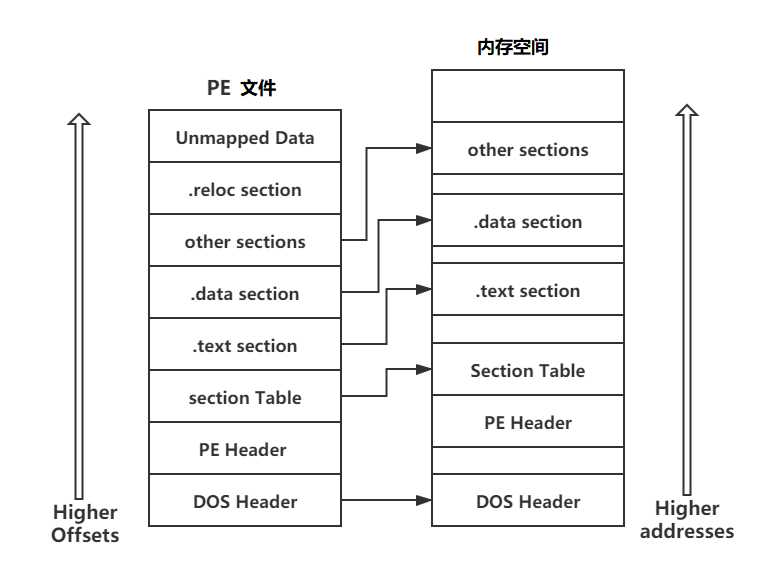
\includegraphics[width=0.9\textwidth]{pememory.png}\\
	\bicaption{PE文件运行后再内存中的节区排布情况}{After the PE file is run, then the section layout in memory}

	\label{sec2:subsec3:pememory}
\end{figure}

%PE文件的结构通常如图\ref{cha2:fig:pefile}所示:



\subsection{DOS MZ Header}

每个PE文件都以一个小型MS-DOS可执行文件开头\cite{向飞2019一种基于}。在Windows的早期,即大量的用户运行它之前,就需要此存根可执行文件\cite{吕苗苗2019基于}。在没有Windows的计算机上执行时,该程序至少可以打印出一条消息,指出要运行该可执行文件是Windows平台上的程序。

PE文件的第一个字节以传统的MS-DOS标头开始\cite{2018Enhance},称为IMAGE\textunderscore DOS\textunderscore HEADER。任何重要的仅有两个值是e\textunderscore magic和e\textunderscore lfanew字段包含PE标头的文件偏移。e\textunderscore magic字段(一个WORD)需要设置为值0x5A4D。这个值有一个\#define,名为IMAGE\textunderscore DOS\textunderscore SIGNATURE。在ASCII表示中,0x5A4D是MZ,MZ是Mark Zbikowski(MS-DOS的原始体系结构之一)的缩写。


\subsection{PE文件头}

PE Header在PE文件中的数据结构名为IMAGE\textunderscore NT\textunderscore HEADERS,IMAGE\textunderscore NT\textunderscore HEADERS结构是存储PE文件详细信息的主要位置。它的偏移量由文件开头IMAGE\textunderscore DOS\textunderscore HEADER中的e\textunderscore lfanew字段给出。IMAGE\textunderscore NT\textunderscore HEADER结构实际上有两个版本,一个用于32位可执行文件,另一个用于64位版本,两个版本的文件结构差异较小\cite{2018Construction}。微软认可的唯一正确的区分两种格式的方法是通过IMAGE\textunderscore OPTIONAL\textunderscore HEADER中的Magic字段的值。

IMAGE\textunderscore NT\textunderscore HEADER由三个字段组成,如图\ref{sec2:subsec3:image_nt_header}。

\begin{figure}[htbp]
	\centering
	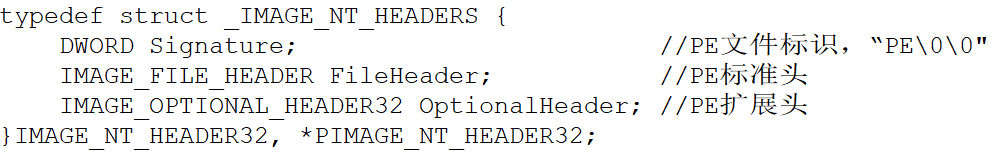
\includegraphics[width=0.9\textwidth]{image_nt_header.png}\\
	\bicaption{IMAGE\_NT\_HEADER结构定义}{IMAGE\_NT\_HEADER structure definition}
	\label{sec2:subsec3:image_nt_header}
\end{figure}

\subsection{相对虚拟地址}

在可执行文件中,有很多地方需要指定内存地址。例如,引用全局变量时需要一个绝对地址。PE文件可能在过程地址空间中的任何位置加载。虽然它们确实具有首选的加载地址,首选加载地址可能已经被使用了,这时的绝对地址就会发生改变\cite{张晓寒2020基于指令虚拟化的安卓本地代码加固方法}。因此,使用某种方式指定可执行文件加载位置的地址非常重要。

为了避免在PE文件中使用硬编码的内存地址,使用了RVA(Relative Virtual Addresses)。RVA只是相对于PE文件加载位置的内存偏移量。例如,考虑一个在地址0x400000加载的EXE文件,其代码段在地址0x401000\cite{何永瑾2020基于注册码的软件授权保护系统的设计与实现}。代码部分的RVA为:

(Target address)0x401000 - (Load address)0x400000  = (RVA)0x1000

要将RVA转换为实际地址,只需完成以下过程即可:将RVA添加到实际加载地址以找到实际的内存地址。实际的内存地址在PE术语中称为虚拟地址。定位VA的另一种方法是,使用首选加载地址的RVA通过上述方法计算得出。

\subsection{区块表}

在PE文件头IMAGE\textunderscore NT\textunderscore HEADERS结构之后的是区块表。IMAGE\textunderscore SECTION\textunderscore HEADERs结构的数组。IMAGE\textunderscore SECTION\textunderscore HEADER提供有关其关联节的信息,包括位置,长度和特征。IMAGE\textunderscore SECTION\textunderscore HEADER结构的数目由IMAGE\textunderscore NT\textunderscore HEADERS.FileHeader.NumberOfSections字段给出。


\subsection{导入表}


在PE文件中,存在名为导入表的数据结构数组,导入表给出了所有需要导入的DLL的名称,并指向一个函数指针数组。函数指针数组称为导入地址表(IAT)。每个导入的API在IAT中都有其自己的保留位置,其中,导入函数的地址由Windows加载程序编写。最后一点特别重要,加载模块后,IAT包含调用导入的API时调用的地址\cite{2018A}。

IAT的优点在于,PE文件中只有一个地方存储了导入的API地址。无论分散通过多少个源文件调用给定的API,所有调用都将通过IAT中的同一函数指针进行\cite{马雪婷2020一种共享软件保护机制的完整实现}。

下面将会通过一个实例来说明导入表的作用,有两种情况需要考虑:直接跳转和间接跳转,在直接跳转中,以执行CALL DWORD PTR [0x00405030]为例,对导入的API调用如图\ref{sec2:subsec3:direct}所示。

\begin{figure}[htbp]
	\centering
	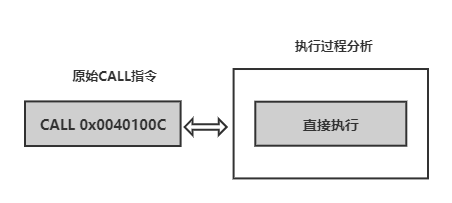
\includegraphics[width=0.6\textwidth]{direct.png}\\
	\bicaption{直接调用过程}{Direct call procedure}
	\label{sec2:subsec3:direct}
\end{figure}

CUP的EIP寄存器将会被设定为0x00405030,对导入的API使用间接跳转调用时,如图\ref{sec2:subsec3:importtable}所示。

\begin{figure}[htbp]
	\centering
	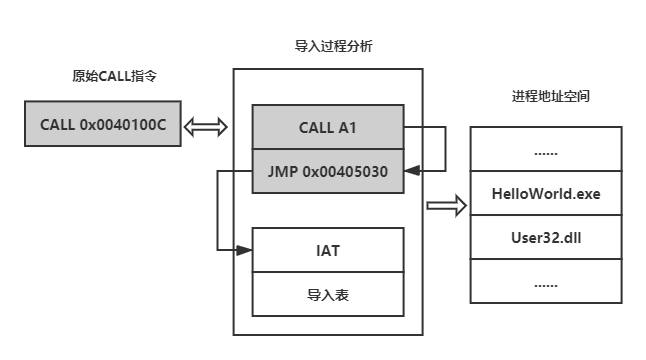
\includegraphics[width=0.9\textwidth]{importtable.png}\\
	\bicaption{使用导入表间接调用过程}{The procedure is called indirectly using the import table}
	\label{sec2:subsec3:importtable}
\end{figure}

执行的指令如下:

CALL 0x0040100C

•••

0x0040100C:

JMP       DWORD PTR [0x00405030]

在这种情况下,CALL将控制权转移到一个中继地址,中继地址中存储着API需要跳转的绝对地址0x405030。0x405030属于IAT中的一项数据。简而言之,效率较低的导入API调用使用了五个字节的附加代码,由于额外的JMP,执行时间更长。

这里使用了一个较低效率的方法来实现CALL指令,这是因为编译器无法区分导入的API调用和同一模块内的普通函数,对于编译器来说,在执行CALL指令时,将会发出如下的指令:CALL XXXXXXXX,其中XXXXXXXX是实际的代码地址,稍后将由链接器填写,这个CALL指令不是通过函数指针进行的,而是一个实际的代码地址,为了让程序正常执行,链接器需要有一段代码来代替XXXXXXXX,最简单的方式是将调用指向JMP存根\cite{2016Building}。

JMP的存根就来自导入函数的导入库,如果检查这个导入库,并且检查如导入的API名称相关的代码,会发现它是一个JMP存根。这意味着默认情况在没有任何干预的情况下,导入的API调用将使用效率较低的形式\cite{2019The}。



PE文件由许多标题和节组成,这些标题和节告诉动态链接程序如何将文件映射到内存中。可执行映像由几个不同的区域组成,每个区域需要不同的内存保护。因此,每个部分的开头必须与页面边界对齐。例如,通常.text节保存程序代码被映射为execute / readonly,而.data部分被映射为不执行/读写。但是,为避免浪费空间,不同部分在磁盘上未按页面对齐。动态链接器的部分工作是根据标题中的说明,将每个部分分别映射到内存,并为生成的区域分配正确的权限。

值得注意的一部分是导入地址表IAT,当应用程序在另一个模块中调用函数时,它用作查找表。它可以采用按序导入和按名称导入的形式。由于编译后的程序无法知道其依赖的库的存储位置,因此,每当进行API调用时,都需要进行间接跳转。当动态链接器加载模块并将它们连接在一起时,它会将实际地址写入IAT插槽,以便它们指向相应库函数的存储位置。尽管这会增加模块内调用的开销,从而导致性能下降,但它提供了一个关键的好处:需要写时复制的内存页数装入程序更改的内容最小化,从而节省了内存和磁盘I / O时间。如果编译器提前知道调用将是模块间的,则可以生成更多优化的代码,这些代码只会导致间接调用操作码。

%
在导入表中,PE文件通常不包含与位置无关的代码。相反,它们被编译为首选的基地址,并且编译器/链接器发出的所有地址都提前固定。如果PE文件无法在其首选地址加载,操作系统将重新修复它。这涉及重新计算每个绝对地址,并修改代码以使用新值。加载程序通过比较首选加载地址和实际加载地址并计算增量值来完成此操作。然后将其添加到首选地址,以提供存储位置的新地址。基地搬迁存储在列表中,并根据需要添加到现有存储位置。现在,生成的代码是该过程专用的,不再可共享,因此在这种情况下,DLL的许多节省内存的好处都丧失了。这也大大降低了模块的加载速度。因此,应尽可能避免重新基准化,Microsoft提供的DLL具有预先计算的基址,以免重叠。因此,在无基准的情况下,PE具有代码效率非常高的优点。这与使用完全与位置无关的代码和全局偏移表的ELF形成对比,后者在执行时间之间进行权衡以降低内存使用量。

在Windows NT操作系统上,PE当前支持x86,IA-32,x86-64(AMD64 / Intel 64),IA-64,ARM和ARM64 指令集体系结构。在Windows 2000之前,Windows NT因此也包括PE支持MIPS,Alpha和PowerPC ISA。由于PE在Windows CE上使用,因此它继续支持MIPS,ARM和SuperH ISA的多个变体。

以上已经对PE文件结构需要修改的地方进行了分析,本文将按照上述内容,对PE文件进行修改,实现反调试加密和虚拟机加壳功能。
\section{PE文件对抗逆向分析的常见方法}

目前市面上的大部分需要都需要软件保护措施,除去普通的方式例如序列号验证、网络注册、花指令等方式,最为普遍的就是软件加壳,软件加壳的根本目的是防止破解者对软件进行逆向分析,从而阻止他们的非法修改和逆向编译,从而保护了上述序列号验证和网络注册等方式,也可以说软件加壳的保护层面更高,如果保护得当,可以从根本上杜绝软件被非法修改。软件保护界也存在一句名言——没有不能脱的壳,所以说本课题研究的抗逆向目标也是在某种程度上加大破解的破解难度,延长他们的破解时间。软件加壳简而言之,将壳与程序通过某种方式混合在一起或进行代码变形,从而让破解者不能正确分辨软件逆向分析无用的壳代码和软件功能流程代码。软件加壳后的程序如图\ref{sec2:subsec3:aftershell}所示。

\begin{figure}[htbp]
	\centering
	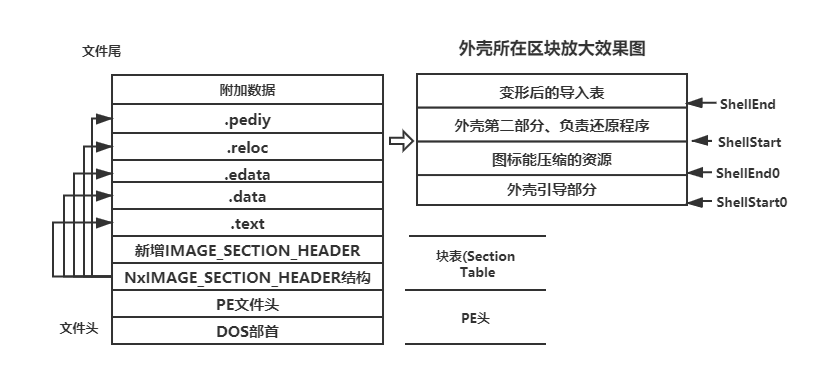
\includegraphics[width=1.0\textwidth]{aftershell.png}\\
	\bicaption{加壳后的程序的结构}{The structure of the program after shell}
	\label{sec2:subsec3:aftershell}
\end{figure}

%\subsection{加壳}
软件加壳按照方法和目的可以分为两大类,第一类是压缩壳,第二类是保护壳。保护壳是本课题的主要研究内容,这种壳的目的是加大破解者的逆向分析难度,代码会将功能代码和外壳代码混淆,可使用密钥对称加密或者非密钥加密两种方式,密钥对称加密则是在软件购买时,商家为用户提供一个私钥,用户只能通过这个私钥打开这个程序,其中的原理与普通的加密算法相仿,但是由于这种方式容易让破解者对私钥和加密代码进行分析,反而减小了破解难度,所以这种方式逐渐被淘汰,非密钥加密则是使用密码学中难以逆向分析的算法对软件进行保护。第二类的压缩壳的目的是为了减小软件的体积,但是由于软件使用了压缩算法,解密和程序运行时同时进行的,会增加程序的运行时间,压缩算法也是不断在优化当中,在时间和空间上进行取舍,这种方式基本没有保护作用,因为压缩壳并不妨碍软件破解者进行逆向分析,利用ESP栈平衡原理,很容易得到软件OEP,修复IAT表后会直接得到解压后的软件,然后再进行破解序列号的逆向分析,所以压缩壳对软件的保护作用形成虚设。

软件加壳按照保护分类可以分为两种方式,一种是本文所采用的虚拟机加壳保护,第二种是采用可执行压缩的方式。所谓可执行压缩是任何手段压缩的可执行文件,并用解压缩代码的压缩数据组合成单个可执行文件。执行此压缩的可执行文件时,解压缩代码会在执行之前从压缩的代码重新创建原始代码。在大多数情况下,压缩的保护方式是透明的,因此可以与原始文件完全相同的方式使用压缩的可执行文件。可执行压缩器通常被称为“运行时打包程序”,“软件打包程序”,“软件保护程序”,甚至是“多态打包程序”和“混淆工具”。压缩的可执行文件可以被视为自解压存档,其中压缩的可执行文件与相关的解压缩代码一起打包在可执行文件中。某些压缩的可执行文件可以解压缩以重建原始程序文件,而无需直接执行。可以用于执行此操作的两个程序是CUP386和UNP。大多数压缩的可执行文件在内存中对原始代码进行解压缩,并且大多数需要更多的内存才能运行因为它们需要存储解压缩器代码,压缩的数据和解压缩的代码。此外,某些压缩的可执行文件还具有其他要求,例如那些在执行前将解压缩的可执行文件写入文件系统的要求。

\subsection{压缩壳}
\label{cha3:sec:mutualdet}

软件程序的压缩壳软件与我们通常意义上的压缩软件如RAR不同,RAR软件压缩之后的文件格式不能被Windows内核程序加载器识别,压缩之后的文件结构已经不是EXE程序,所以不能成功运行。

压缩壳的产生时间较早,早在DOS时代,受到当时的硬件设备的限制,计算机的内存和硬盘需要严格计划使用,也受到移动存储介质的限制,软件开发者不得不想出办法来减小应用软件的占用空间,于是程序压缩技术产生了。对可执行文件进行压缩后,其内部的功能代码结构大部分发生改变,其中的汇编代码和硬编码地址已经和初始状态不能直接进行反汇编,加大了破解难度,起到了一定的反破解作用。压缩同一款产品,压缩比例越高,程序的功能代码变化越大,破解的难度也会随之提高。

压缩算法通常是使用市面上的压缩引擎,由于解压和程序的运行是同时进行的,解压会增加程序的运行时间,所以解压效率是衡量一款解压算法的重要标志,压缩的速度可以慢下来,但是解压速度需要不断的提高,如果解压速度太慢会影响用户体验。有代表性的压缩壳有ASPack、UPX和PECompact等。

ASPack是Windows下的应用程序压缩软件,市面上很多软件都使用这款压缩软件,但是由于使用用户太多,导致研究的人也多,其中的保护作用已经越来越来,现在用这款软件的目的大部分是为了减小应用软件的体积,压缩壳通常可以将可执行文件和其他依赖文件打包在一起压缩,从而减少了文件的数量,ASPack压缩后的程序是后缀为EXE的可执行文件,压缩后的程序可直接运行,并且程序的运行并不依赖ASPack这款软件,这也是与普通压缩软件差别最大的地方。

UPX(Ultimate Packer for eXecutables)是一款针对Windows的对可执行文件进行加密的文件压缩器,压缩率高达50-70$\%$,大大减小了可执行文件的磁盘占用空间,同时也减小了移动介质和网络之间的传输时间。通过UPX压缩过的程序同ASPack软件一样,不会产生功能损失会和压缩之前一样运行。其运行界面如图\ref{sec2:subsec3:upxshell}所示。

\begin{figure}[htbp]
	\centering
	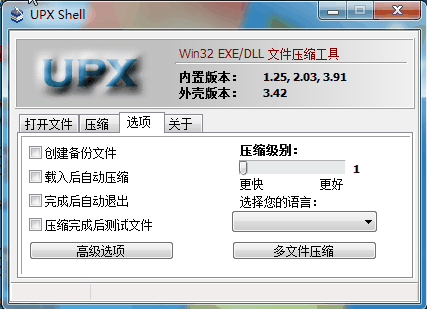
\includegraphics[width=0.7\textwidth]{upxshell.png}\\
	\bicaption{UPX加壳工具}{UPX shell tool}
	\label{sec2:subsec3:upxshell}
\end{figure}

\subsection{保护壳}
\label{cha3:sec:protectshell}
随着脱壳技术的发展,压缩壳的保护性能已经不能满足人们的需要,上述ASPack、PECompact、UPX等压缩壳软件已经形成专门针对的软件,使用压缩壳的应用程序都可以被一键脱壳,调试技术也不断提高,产生了诸多的反汇编工具ODdbg、IDA Pro等、调试工具SoftICE、OllyDbg等,随着硬件设备的性能不断提高,应用程序的占用空间和运行时间已经不是安全问题的瓶颈,防止软件被逆向、反调试技术已经成为研究的重点。于是,在加壳软件中会加入反调试的代码,比如化指令、结构异常处理机制、加密算法、代码混淆等技术,抗逆向技术在不断发展。

保护壳可以自动给应用程序添加安装包保护性外壳程序,并强制在应用程序运行之前确认安全令牌的存在和状态。保护壳还会对软件中的代码和数据进行加密,以防止进行逆向功能,使用这种保护方法,可以在不修改源代码的情况下应用软件保护。有代表性的保护壳有ASPprotect、ACProtect、Armadillo等。

ASProtect是主要面向Windows用户的软件加壳保护软件,这款软件通过RSA加密算法生成唯一KEY,通过对称加密的方式,为用户分配私钥,只有得到私钥的用户,才能在程序运行时对加密功能代码进行正确解密。内置反调试引擎,自己有一套反调试系统,在运行时会开启一个线程,检测自身是否被调试,如果被调试,则直接中断程序,给破解者的破解带来难度。其运行界面如图\ref{sec2:subsec3:asprotect}

\begin{figure}[htbp]
	\centering
	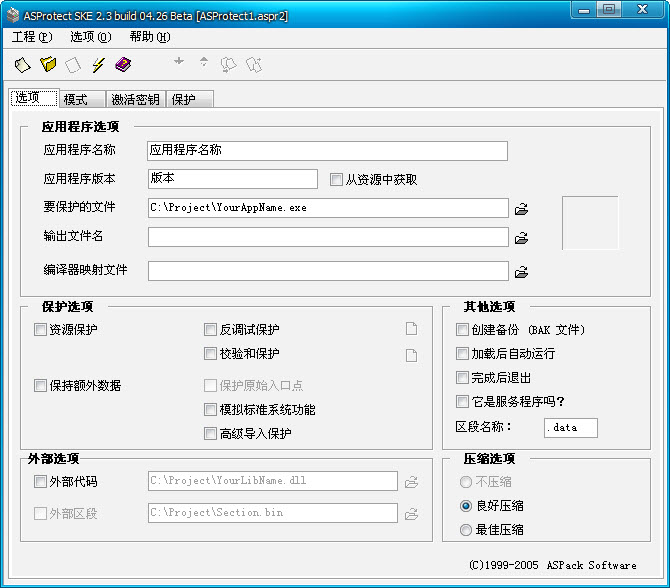
\includegraphics[width=0.8\textwidth]{asprotect.jpg}\\
	\bicaption{ASProtect加壳工具}{ASProtect packing tool}
	\label{sec2:subsec3:asprotect}
\end{figure}

\subsection{工具脱壳}

被加壳软件在运行时是需要脱壳后才会正常执行,软件脱壳就是软件加壳的逆向操作。根据脱壳方式的不同,脱壳方式分为手工脱壳和工具脱壳,工具脱壳通常只适应于流行的加壳软件,越是流行的加壳工具,研究它的人越多,拥有高技术的破解者则可以完全研究明白加壳机制后,写出自动化脱壳机,但是这种自动化脱壳机通常只针对压缩壳。

工具脱壳通常主要分为两类:专业脱壳软件和通用脱壳软件。专业脱壳软件通常只针对一种或两种加壳软件,由于是针对性的软件,脱壳成功率也相对较高。通用脱壳软件通常针对保护性能低的压缩壳,它具有通用性,可以脱掉多种不同的壳。常见的脱壳软件有UnPECompact、UnASPack、UPXShell等。

\subsection{手工脱壳}

通常的压缩壳,都有对应的自动脱壳机,但只针对于压缩壳,由于保护壳的机制太过复杂,
很难写出自动脱壳机,所有保护壳通常需要手工脱壳。

要想手工脱壳需要对PE文件以及程序加载后在内存中的数据非常了解。软件加壳技术的发展总是伴随着脱壳技术的进步,要研究脱壳技术,首先要分析壳的加载过程。壳的加载过程可以分为五个步骤,定位壳需要的所有API地址、解密函数对块(Section)的操作、重定位、EIP设置为OEP(Original Entry Point)、HOOK-API,在程序被脱壳之后,加壳进程将会把CPU的控制权还给原程序,此时原程序就会像没有加壳时的状态正常运行,原本被加密过的各种节区块都会被还原。而此时,则是脱壳程序最关键的时机,此时的程序在内存中的形态和程序没有被加壳过的形态几乎完全一致\cite{2018Method}。

手动脱壳通常分为三个步骤:一是找到程序真正入口点OEP;二是dump下内存映像文件;三是输入表的重建过程。



\subsection{壳的类型分析}

在手工脱壳之前,通常要对软件进行加壳分析,一是分析是否加了壳,二是可以分析出此程序使用了哪种壳或者本程序是用哪种语言编写。这时通常使用市面上流行的PEiD或者FileInfo等工具。PEiD的图形界面如图\ref{sec2:subsec3:peid}所示。

\begin{figure}[htbp]
	\centering
	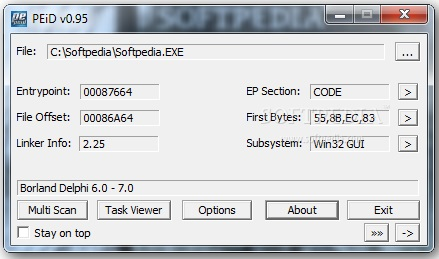
\includegraphics[width=0.8\textwidth]{peid.jpg}\\
	\bicaption{PEiD侦壳工具}{PEiD debugger}
	\label{sec2:subsec3:peid}
\end{figure}

将程序加载到PEiD中,此程序通常会给出很多有用的信息,比如壳的类型和本程序使用的编译器。此程序使用特征码做出识别判断,每种壳都有固定的特征码,只要文件搜索特征码,大部分情况下都可以识别成功,但是对于那种小众加壳或者未被公布的加密壳却无能为力,这也是本课题最终的研究目标。本软件提供了一个扩展接口USERDB.txt,用户可以自定义一些已知的特征码,通过这种方式可以识别出大部分的壳。

加壳与脱壳总是在不断博弈中,正因为PEiD是使用特征码方式识别加壳类型,加壳软件也可以伪造特征码,比如加壳软件在壳中放入多种不同类型的加壳软件特征码,这时PEiD就会失去它的作用,这种方式也被称为"PEiD欺骗”。
%%%%%%%%%%%%%%%%%%%%%%%%%%%%%%%%%%%%%%%%%
%添加一点东西,是之到下一行
\section{本章小节}
本章节对虚拟机加壳和二进制代码混淆的相关技术进行了阐述,并对PE文件结构进行了分析,对其中的DOS头、PE Header、相对虚拟地址等重要结构进行了详细阐述,并简要说明了反调试的原理,说明了在汇编语言和硬编码语言的层面上对Windows下的执行文件进行修改的相关技术,从而可以保证修改文件的正确性和可重用性。